\documentclass[
	a4paper,
	oneside,
	BCOR = 10mm,
	DIV = 12,
	12pt,
	headings = normal,
]{scrartcl}

%%% Length calculations
\usepackage{calc}
%%%

%%% Support for color
\usepackage{xcolor}
\definecolor{lightblue}{HTML}{03A9F4}
\definecolor{red}{HTML}{F44336}
%%%

%%% Including graphics
\usepackage{graphicx}
%%%

%%% Font selection
\usepackage{fontspec}

\setromanfont{STIX Two Text}[
	SmallCapsFeatures = {LetterSpace = 8},
]

\setsansfont{IBM Plex Sans}[
	Scale = MatchUppercase,
]

\setmonofont{IBM Plex Mono}[
	Scale = MatchUppercase,
]
%%%

%%% Math typesetting
\usepackage{amsmath}

\usepackage{unicode-math}
\setmathfont{STIX Two Math}
%%%

%%% List settings
\usepackage{enumitem}
\setlist[enumerate]{
	label*      = {\arabic*.},
	leftmargin  = *,
	labelindent = \parindent,
	topsep      = 1\baselineskip,
	parsep      = 0\baselineskip,
	itemsep     = 1\baselineskip,
}

\setlist[itemize]{
	label*      = {—},
	leftmargin  = *,
	labelindent = \parindent,
	topsep      = 1\baselineskip,
	parsep      = 0\baselineskip,
	itemsep     = 1\baselineskip,
}

\setlist[description]{
	font        = {\rmfamily\upshape\bfseries},
	topsep      = 1\baselineskip,
	parsep      = 0\baselineskip,
	itemsep     = 0\baselineskip,
}

%%%

%%% Structural elements typesetting
\setkomafont{pagenumber}{\rmfamily}
\setkomafont{disposition}{\rmfamily\bfseries}

% Sectioning
\RedeclareSectionCommand[
	beforeskip = -1\baselineskip,
	afterskip  = 1\baselineskip,
	font       = {\normalsize\bfseries\scshape},
]{section}

\RedeclareSectionCommand[
	beforeskip = -1\baselineskip,
	afterskip  = 1\baselineskip,
	font       = {\normalsize\bfseries\itshape},
]{subsection}

\RedeclareSectionCommand[
	beforeskip = -1\baselineskip,
	afterskip  = 1\baselineskip,
	font       = {\normalsize\bfseries},
]{subsubsection}

\RedeclareSectionCommand[
	beforeskip = -1\baselineskip,
	afterskip  = -0.5em,
	font       = {\normalsize\mdseries\scshape\addfontfeatures{Letters = {UppercaseSmallCaps}}},
]{paragraph}
%%%

%%% Typographic enhancements
\usepackage{microtype}
%%%

%%% Language-specific settings
\usepackage{polyglossia}
\setmainlanguage{ukrainian}
\setotherlanguages{english}
%%%

%%% Captions
\usepackage{caption}
\usepackage{subcaption}

%\DeclareCaptionLabelFormat{closing}{#2)}
%\captionsetup[subtable]{labelformat = closing}

%\captionsetup[subfigure]{labelformat = closing}

\captionsetup[table]{
	aboveskip = 0\baselineskip,
	belowskip = 0\baselineskip,
}

\captionsetup[figure]{
	aboveskip = 1\baselineskip,
	belowskip = 0\baselineskip,
}

\captionsetup[subfigure]{
	labelformat = simple,
	labelformat = brace,
}
%%%

%%% Hyphenated ragged typesetting
\usepackage{ragged2e}
%%%

%%% Table typesetting
\usepackage{booktabs}
\usepackage{longtable}

\usepackage{multirow}

\usepackage{array}
\newcolumntype{v}[1]{>{\RaggedRight\arraybackslash\hspace{0pt}}p{#1}}
\newcolumntype{b}[1]{>{\Centering\arraybackslash\hspace{0pt}}p{#1}}
\newcolumntype{n}[1]{>{\RaggedLeft\arraybackslash\hspace{0pt}}p{#1}}
%%%

%%% Drawing
\usepackage{tikz}
\usepackage{tikzscale}
\usetikzlibrary{positioning}
\usetikzlibrary{arrows.meta} % Stealth arrow tips
%%%

%%% SI units typesetting
\usepackage{siunitx}
\sisetup{
	output-decimal-marker = {,},
	exponent-product      = {\cdot},
	inter-unit-product    = \ensuremath{{} \cdot {}},
	per-mode              = symbol,
}
%%%

%%% Keystroke and menus typesetting
\usepackage{menukeys}
%%%

%%% Links and hyperreferences
\usepackage{hyperref}
\hypersetup{
	bookmarksnumbered = true,
	colorlinks      = false,
	linkbordercolor = red,
	urlbordercolor  = lightblue,
	pdfborderstyle  = {/S/U/W 1.5},
}
%%%

%%% Length adjustments
% Set baselineskip, default is 14.5 pt
\linespread{1.068966} % ~15.5 pt
\setlength{\emergencystretch}{1em}
\setlength{\parindent}{1.5em}
\newlength{\gridunitwidth}
\setlength{\gridunitwidth}{\textwidth / 12}
%%%

%%% Custom commands
\newcommand{\allcaps}[1]{{\addfontfeatures{LetterSpace = 8, Kerning = Off}#1}}
\newcommand{\Mytextrightarrow}{$\rightarrow$\hspace{0.25em}}
\newcommand{\key}[1]{\textsf{#1}}
%%%

\begin{document}

\begin{titlepage}
		\begin{center}
			Міністерство освіти і науки України\\
			Національний авіаційний університет\\
			Навчально-науковий інститут комп'ютерних інформаційних технологій\\
			Кафедра комп'ютеризованих систем управління

			\vspace{\fill}
				Лабораторна робота №1.2~(частина~2)\\
				з дисципліни «Технології мультимедіа»\\
				на тему «Виділення фрагментів зображення»\\

			\vspace{\fill}

			\begin{flushright}
				Виконав:\\
				студент \allcaps{ННІКІТ}\\
				групи СП-325\\
				Клокун В.\,Д.\\
				Перевірив:\\
				Кашкевич І.\,Ф.
			\end{flushright}

			Київ 2018
		\end{center}
	\end{titlepage}

	\section{Мета роботи}
		Вивчити основні інструменти програми~\textenglish{Adobe Photoshop} для~кадрування цифрових зображень.

	\section{Завдання роботи}
		Навчитися використовувати інструменти \emph{\textenglish{Image}~\Mytextrightarrow \textenglish{Crop}} для~кадрування зображень; вивчити можливість інвертування зображення; ознайомитися з~інструментами для~переміщення, дублювання і~редагування області виділення зображення.

	\section{Хід роботи}
		\subsection{Виділення прямокутних ділянок}
			Створюємо новий документ та~додаємо прямокутну область. Для~цього виділяємо прямокутну область і~заливаємо~її кольором. До~створеного прямокутника додаємо контур~(рис.~\ref{fig:01-rectangle-res})

			\begin{figure}[!htbp]
				\centering
				
\includegraphics[height = 6\baselineskip]{./../01-solution/y03s01-multimedia-lab-02-02-p01.jpg}
				\caption{Отриманий прямокутник}
				\label{fig:01-rectangle-res}
			\end{figure}

		\subsection{Виділення еліптичних областей}
			Додаємо еліптичну область, для цього виділяємо і~заливаємо~її кольором~(рис.~\ref{fig:02-ellipse-res})

			\begin{figure}[!htbp]
				\centering
				
\includegraphics[height = 5\baselineskip]{./../01-solution/y03s01-multimedia-lab-02-02-p02.png}
				\caption{Отриманий еліпс}
				\label{fig:02-ellipse-res}
			\end{figure}

		\subsection{Виділення елементів об'єкта зі~зміною фону}
			Виділяємо об'єкт за~допомогою зручного інструмента виділення, інвертуємо виділену область за~допомогою комбінації клавіш~\key{\textenglish{Ctrl}}~+ \key{\textenglish{Shift}}~+ \key{\textenglish{I}} та~видаляємо виділену область натиском клавіші~\key{Del}~(рис.~\ref{fig:03-bg-change-res}).

			\begin{figure}[!htbp]
				\centering
				
\includegraphics[height = 4\baselineskip]{./../01-solution/y03s01-multimedia-lab-02-02-p03.png}
				\caption{Результат виділення елементів об'єкта зі~зміною фону}
				\label{fig:03-bg-change-res}
			\end{figure}

		\subsection{Виділення за допомогою «чарівної палички»}
			Виділяємо об'єкт за~допомогою чарівної палички, інвертуємо виділену область за~допомогою комбінації клавіш~\key{\textenglish{Ctrl}}~+ \key{\textenglish{Shift}}~+ \key{\textenglish{I}}.~(рис.~\ref{fig:04-magic-wand-res})

			\begin{figure}[!htbp]
				\centering
				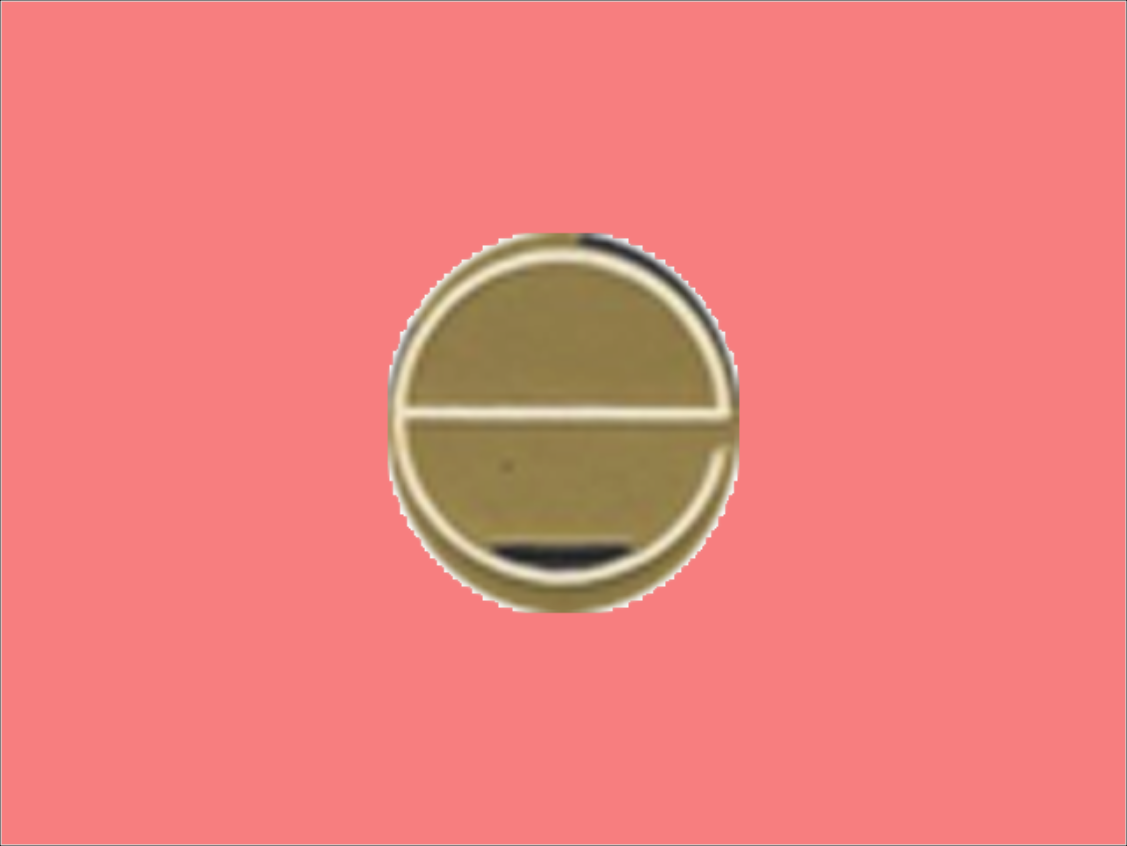
\includegraphics[height = 4\baselineskip]{./../01-solution/y03s01-multimedia-lab-02-02-p04-v03.png}
				\caption{Результат виділення за допомогою «чарівної палички»}
				\label{fig:04-magic-wand-res}
			\end{figure}

		\subsection{Виділення за~допомогою полігонального ласо. Переміщення, копіювання і~редагування області виділення}
			Виділяємо об'єкт за~допомогою інструмента~\emph{\textenglish{Polygonal Lasso}}, копіюємо його за~допомогою комбінації клавіш~\key{\textenglish{Ctrl}}~+ \key{\textenglish{C}}, переміщуємо за~допомогою миші та~трансформуємо за~допомогою клавіш~\key{\textenglish{Ctrl}}~+ \key{\textenglish{T}}~(рис.~\ref{fig:05-polygonal-lasso-res}).

			\begin{figure}[!htbp]
				\centering
				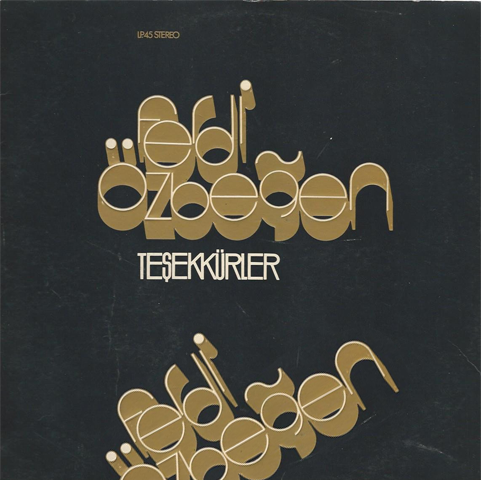
\includegraphics[height = 4\baselineskip]{./../01-solution/y03s01-multimedia-lab-02-02-p05.png}
				\caption{Результат виділення за~допомогою полігонального ласо, переміщення копіювання і~редагування}
				\label{fig:05-polygonal-lasso-res}
			\end{figure}

	\section{Висновок}
		Виконуючи дану лабораторну роботу ми~вивчили основні інструменти програми~\textenglish{Adobe Photoshop} для~кадрування цифрових зображень.

\end{document}
